\documentclass{article}
\usepackage[utf8]{inputenc}
\usepackage{latexsym}
\usepackage[rightcaption]{sidecap}
\usepackage{wrapfig}
\usepackage{url}
\usepackage{graphicx}
\usepackage{hyperref}
\usepackage{array}
\usepackage[table]{xcolor}
\usepackage{multirow}
\hypersetup{colorlinks=true}
\usepackage{enumitem,amssymb}
\usepackage{enumerate}
\newlist{todolist}{itemize}{4}
\setlist[todolist]{label=$\square$}



\title{Latex-Analiza Complexit\u {a}\c {t}ii }
\author{Constantin Ionu\c {t} Andrei }
\date{May 25, 2017}

\begin{document}

\maketitle
\large{
{Instruc\c{t}iuni simple complexitate O(1)}

a = a + 1

a $>$ 0

a - 1

\underline{Instruc\c{t}iunea if}

if conditie  \{     \hspace{100}         complexitate q+1

  \hspace{13} ......... 
   
  \hspace{13} ......... \} $=>$ q
  
  \} else \{
  
  \hspace{13} .........
  
  \hspace{13} .........  p \hspace{100} complexitate p+1
  
  \}
  
  Instruc\c{t}iunea switch
  
  Switch \hspace{7} x \hspace{7} \{ \hspace{70} Complexitate fara break=
  
  \hspace{22} case 1: ...... \hspace{60} nr case $+$ complexitate true
  
  \hspace{22} case 2: ...... \hspace{75} sau complexitate default
  
   
  
  \hspace{22} case 3 : ..... \hspace{60} complexitate cu break
  
  \hspace{22} default : .... \hspace{75} aceeasi si de mai sus daca
  
  \hspace{170} nu sunt multiple cazuri
  
  \}
  
  \hspace{22} switch \hspace{7} x \hspace{7} \{
  
  \hspace{14} case 2: ..... break
  
  \hspace{14} case 2: .....
  
  \hspace{14} default: .....
  
  \}
  
  \pagebreak
  
  \underline{Instruc\c{t}iunea while}...
  
  \hspace{30} conditie
  
  while $(x \leq n)$ \{ \hspace{80} Complexitate: nr\hspace{4}pasi x $(q+1)$ 
  
  \hspace{30} ....... \\
  
  \hspace{30} ........ q \\
  
  \hspace{30} ........ \\\\
  
  \}
  
  \underline{Instruc\c{t}iunea do...while}
  
  do \{
  
  \hspace{7} ......
  
  \hspace{7} ...... q \hspace{90} Complexitate
  
  \hspace{7} ...... \\\\
  
  \} while(conditie)
  
  $x=0;$
  
  do \{ \hspace{90} $(nr\hspace{4} pasi)$ $(q+1)$
  
  \hspace{4} $x=x+1;$
  
  \} while $(x \leq 3);$ \\\\
 
 
  
  x=1 \hspace{35} x=4
  
  
  comp true \hspace{7} comp false \\
  
  $x=2$
  
  com true
  
  $x=3$
  
  comp  true
  
  \pagebreak
  
  \underline{ Instruc\c{t}iunea \hspace{14} for} \\\\
  
  for $(start , stop , increment)$ \{
  
  \hspace{7} ..........
  
  \hspace{7} ..........  \hspace{4} q \\\\
  
  \}  \hspace{60} Complexitate: $1+ nr\hspace{4} pasi$ x $(q+2)$
  
  ---------------------------------------------------------------------------------------\\\\
  
   \hspace{7} for $(i=0 ; i \leq 100 ; i=i+2)$ \{
  
   \hspace{14} if $(i\%10==0)$ \{  \hspace{46} nr pasi$=$51
   
    \hspace{22} print .......
    
   \hspace{14}  \}
    
    \}   \hspace{170} $1+51 (+)$ \\
    
    -----------------------------_ \hspace{40} $1+11(1+1)+40x1$
   \\  
     
   Ordinul complexitatii   \hspace{40} $=1+22+40=63$    complexitate \\
   
   -O$(1)$ \\
   
   -O$(log \hspace{2} n)$ logaritmica   \hspace{40} $1+(\frac{n}{2}+1)(+)$ \\
   
   -O$(n)$ liniara \\
   
   -O$(n^{2})$ patratic \hspace{60} $1+\frac{4n}{10}$x$1+(\frac{n}{10}+1)$x$2$ \\
   
   -O$(n^{3})$ cubic \hspace{50} --------------------------------------- \\
   
   -O$(x^{n})$ exponential  \hspace{50} Complexitatea se calculeaza pentru 
   
   \hspace{160} n $->$ \infty
   
   \hspace{160} - input max
   
   \pagebreak
   
   O$(n)$ \hspace{7} "big OH" \hspace{7} -limita superioara -\hspace{4} upper bound \\
   
   O$(g(n))$\hspace{3}= \hspace{3}\{ $f(n): E_{c}$,\hspace{4} n_{0} \hspace{7} a.i. f$(n)\leq g(n)$, \hspace{7}$n \geq n_{0}$ \}\\
   
   f$(n)$ = $5n^2+2n+1$\hspace{7}=\hspace{7}O$(n^2)$ \hspace{12} C=$5+2+1$
   
   \hspace{172} n_{0} = 1 \\\\
   
   f$(n) \leq 8n^2$ \\
   
 \fbox { f$(n) \leq Cn^2$ \hspace{7},\hspace{7} n$\hspace{7}\geq \hspace{7} n_{0}$ } \\\\\\\\\\\\\\\\\\\\\\\\\\\\
 
 \Omega - Omega \hspace{17} -limita \hspace{4} inferioara \hspace{14} lower \hspace{4} bound \\
 
 \Omega $(g(n))$ \hspace{7} = \{ f$(n)$ :\hspace{7} \exists \hspace{7} C, \hspace{7} n_{0}\hspace{7} a.i.\hspace{7} g$(n)$
 
 \hspace{97} \geq f$(n)$, \hspace{7} n \leq n_{0} \} \\
 
 f$(n)$ = $5n^2+2n+1$=$\Omega(n^2)$ \\
 
 C = 5
 n_{0} \hspace{60} $5n^2+2n+1 \geq 5n^2 \hspace{7} pt\hspace{7} n \geq 0$ \\
 
 \pagebreak
 
 \theta \hspace{4}-\hspace{4}Theta\hspace{7} - growth\hspace{7} \hspace{7}of\hspace{7} function \hspace{7}f \\\\\\\
 
 \theta\hspace{4} $(g(n))$\hspace{7}=\hspace{7}$ \{ f(n):\hspace{7} \exists\hspace{7} C_{1},\hspace{7}C_{2},\hspace{7}n_{0}$\hspace{14} a.i. \\\\\\\\\
 
 \hspace{40}C_{1}$g(n)$ \leq\hspace{7} $f(n)$ \leq\hspace{7} C_{2}$g(n)$, \hspace{7} n \geq n_{0} \} \\\\\\\
 
 $f(n)$\hspace{7}= \hspace{7} $5n^2+2n+1$\hspace{7}=\hspace{7}
 \theta$(n^2)$ \\\\\\\\\
 
 \hspace{14}C_{1}=5 \hspace{14} C_{2}=8 \hspace{14} n_{0}=1 \\\\\\\\\\\
 
 \hspace{50} $5n^2 \leq\hspace{7}5n^2+2n+1\leq\hspace{7}8n^2$ pt n \geq 1 \\\\\\\\
 
 \pagebreak
 
 procedure bubbleSort$(A)$ \\
 
\hspace{7} n = length$(A)$ \\
 
\hspace{7} repeat\\
 
 \hspace{7}\hspace{9} swapped = false \hspace{200} O$(1)$\\
 
 \hspace{7}\hspace{9} for i = 1\hspace{7}to\hspace{7}$n-1$\hspace{7}do \\
 
 \hspace{7}\hspace{7}\hspace{7}\hspace{7}\hspace{7}if $A[i-1]>A[i]$ then \\
 
 \hspace{7}\hspace{7}\hspace{7}\hspace{7}\hspace{7}\hspace{7}\hspace{7} swap $(A[i-1],A[i])$ \hspace{157} O$(3)$ \\
 
 \hspace{49} swapped\hspace{7}=\hspace{7}true \hspace{163} O$(1)$ \\
 
 \hspace{7} until\hspace{14} not \hspace{14} swapped \\\\
 
 $[1+(n-1)(5+2)+1]\hspace{7}(n-1)$ \\
 
 =\hspace{7}$7(n-1)^2+2n-2$\hspace{7}=\hspace{7}$7(n^2-2n+1)+2n+2$\\
 
 \hspace{20} o_{1}\hspace{7}o_{2}\hspace{7}.........\hspace{7}o_{n-1}\hspace{50} o_{n}=\fbox{$7n^2-12n+3$} 
 
 \hspace{71}$(n-1)$ swaps required in worst case \\
 
 1 repeat  
 
 \hspace{140} 2 repeat \hspace{50} 3 repeat \\
 
 I \hspace{7} 4 3 2 1 \hspace{70} I\hspace{14}3 2 1 4 \hspace{40} I\hspace{14} 2 1 3 4 
 
  II\hspace{7} 3 4 2 1 \hspace{70}II\hspace{14}2 3 1 4 \hspace{40}II\hspace{14} 1 2 3 4 
  
   III\hspace{7}3 2 4 1 \hspace{70}III\hspace{10}2 1 3 4
   
   IV\hspace{7}3 2 1 4 
   
   \pagebreak
   
   O$(n)\hspace{4}$=$\hspace{4}7n^2=\hspace{4}O(n^2)$ 
   
   \Omega$(n)\hspace{4}=\hspace{4}6n^2$\hspace{11}pt n\approx$\hspace{4}6+\sqrt{33}\hspace{4}\approx\hspace{4}13,75\hspace{4}$=O$n^2)$ \\
   
   \hspace{40}$7n^2-12n+3=7n^2$\\
   
   \hspace{48}$-12n+3=0$\\
   
   \hspace{48}$3=12n => n=\frac{3}{12}=\frac{1}{4}$\\
   
   \hspace{40}$7(\frac{1}{4})^2-12\frac{1}{4}+3=7\frac{1}{16}-3+3$ \\
   
   \hspace{40}$=\frac{7}{16}$ \hspace{140} \fbox{$7n^2-12n+3=5n^2$}
   
   \hspace{40}$7n^2-12n+3=6n^2$ \hspace{60} \fbox{$2n^2-12n+3=0$} \\
   
   
   
  \\
  
  

$\Delta$ = $b^2 - 4 * a*c$ \\

$\Delta$ = $144-12$ \\ 

$\Delta$ = 132 \\

$x{_1} = \frac{-b+\sqrt\Delta}{2*a}$  = $\frac{12 + \sqrt 132}{2}$ = $6 + \sqrt 33$ $\simeq$ $6 + 5,75 = 13,75$ \\ 

O(n) \ \ \ \ \  \ \ \ \ $6*n^2 \leq f(n) \leq 7*n^2 $ \\ 
O(n) = $n^2$ \ \ \ \ \ \ $7*n^2 - 12*n + 3 = 5*n^2$ \\
\indent \hspace{1.9cm}{$2*n^2-12*n+3=0$} \\
\indent \hspace{1.9cm}{$\Delta$ $= 144-24 =  120$} \\
\indent \hspace{1.9cm}{$x{_2}$ = $\frac{12+\sqrt 120}{4}$ = $3+\frac{\sqrt 120}{4}$} \\ 


\pagebreak

{\bf recursive}

\begin{figure}[ht]
\begin{center}
\begin{tabbing}

\indent \bf Factorial \\
\indent f(n) \=\{ \\
\indent \> if n=0 return 1 \hspace{1cm}{\it O(1)}\\
\indent \> else return n*f(n-1) \\
\indent \} \\
\end{tabbing}
\label{fig_alg_ex}
\end{center}
\end{figure}

\begin{figure}[ht]
\begin{center}
\begin{tabbing}

\indent T(n) \== T(n-1) + 3 \ \ \ \ \ $n \geq 0$ \\
\indent \>=T(n-2) + 6 \\
\indent \>=T(n-3) + 9 \\
\indent \>=T(n-k) + 3*k \\

\indent T(0) $\Rightarrow$ \=n-k=0 $\Rightarrow$ k=n \\
\indent \>T(n) = T(0) + $3*n = 1+3*n$ = O(n)\\


\end{tabbing}
\label{fig_alg_ex}
\end{center}
\end{figure}

\begin{figure}[ht]
\begin{center}
\begin{tabbing}
\indent {\bf Fibonaci} \\
\indent Fib(n\=) \{ \\
\indent \>if n $\leq$ 0\ return\ 1 \\
\indent \>else return Fib(n-1) + Fib(n-2) \hspace{1.9cm}{\it O(1)}\\
\indent \} \\
\indent \\
\indent \\


\end{tabbing}
\label{fig_alg_ex}
\end{center}
\end{figure}

\begin{figure}[ht]
\begin{center}
\begin{tabbing}

\indent $T(n) = T(n-1) + T(n-2) +4$ \\
\indent $T(0)=T(1)=1$ \\
\indent \dots \dots \dots \dots \dots \dots \dots \dots \dots \dots 
\\
\indent Presupunem \=T(n-1) = T(n-2) dar T(n-1) $\geq$ T(n-2)\
approximare\ in\ jos\,\ c\ = 4\ constant\u a \\
\indent \>$T(n) $\==$ 2*T(n-2)+4$ \\
\indent \>\>$=2*(2*T*(n-4)+c)+c$ \\
\indent \>\>$=4*T(n-4)+3*c)$ \\
\indent \>\>$=8*T(n-6) + 7*c)$ \\
\indent \>\>$=16*T(n-8) + 15*c)$ \\
\indent \>\>$=2^k * T*(n-k) + (2^k-1)*c$ \\ 
\indent \>$T(0) => n - 2*k = 0 => k = n/2$ \\
\indent \>$T(n) = 2^{n/2} * T(0)+(2^{n/2}-1)*c$ \\
\indent \>\>=$2^{n/2}*(1+ c) -c$ \\
\indent \>$T(n) = 2^{n/2}$ \ \ \ \ $\Omega$($2^{n/2})$
\indent \\
\indent  \\
\indent Presupunem \=T(n-1) = T(n-2) dar T(n-1) $\leq$ T(n-2)\ deci maximizam functia \\ 
\indent $T(n) $\==$ 2*T*(n-1) + c$ \ \ \ \ \ \ \ c = 4 \\
\indent \>=$2*(2*T(n-2) + c) +c$ \\
\indent \>=$4*T(n-2) + 3*c$ \\
\indent \>=$8*T(n-3) + 7*c$ \\
\indent \>=$2^k*T(n-k)+(2^k-1)*c$ \\
\indent $T(0) => k=n => T(n) * 2^n*T(0)+(2^n-1)*c$ \\
\indent $T(n) = 2^n*T(0) + 2^n*c-c$ \\
\indent \>=$2^n*(T(0) + c) - c$ \\
\indent \>=$2^n*(1+c) - c $ \\
\indent $O(n) = 2^n$

\end{tabbing}
\label{fig_alg_ex}
\end{center}
\end{figure}

\begin{figure}[ht]
\begin{center}
\begin{tabbing}

\indent {\bf Fibo non-recursive} \\
\indent int \=fibo(n) \{ \\
\indent \>if(n$\leq$1) return 1 \\
\indent \>rez = 1 \hspace{3.5cm}{\it O(n)} \\
\indent \>rezPre = 1 \\
\indent \>for i=\=2,n \\
\indent \>\>temp = rez \\
\indent \>\>rez = rez + rezPre \\
\indent \>\>rezPre = temp \\
\indent \>return rez \\
\indent \}
\end{tabbing}
\label{fig_alg_ex}
\end{center}
\end{figure}


\begin{figure}[h]
\centering
\caption{Graph 1}
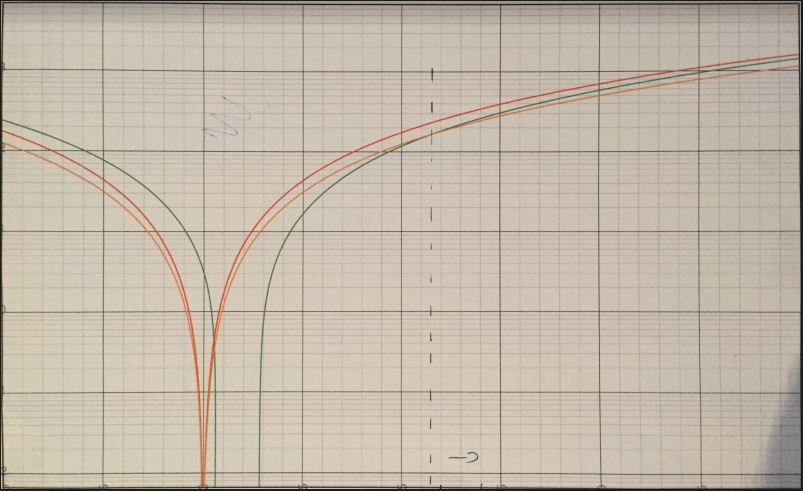
\includegraphics[width=1.2\textwidth]{graph1}
\end{figure}

\begin{figure}[h]
\centering
\caption{Graph 2}
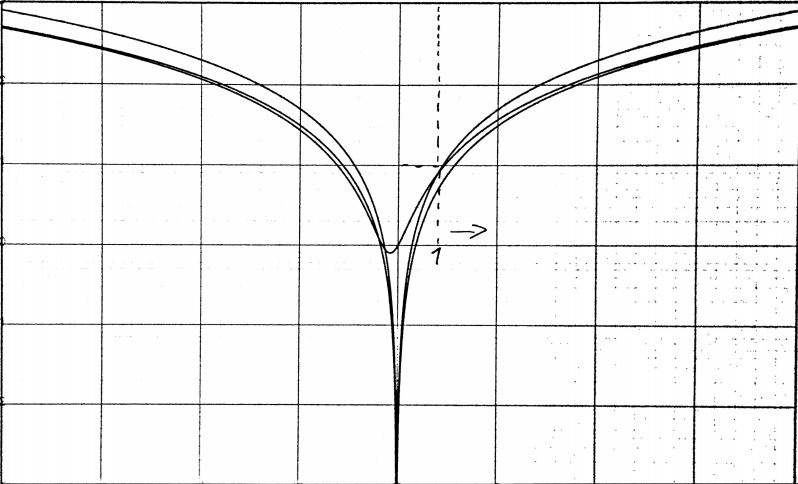
\includegraphics[width=1.2\textwidth]{graph2}
\end{figure}



 
   
   
  
  
 
 
 
 
 
 
 
 
 
 
 
 
 
 
 
 
 
 
 
 
 
 
 
 
 
 
 
 
 
 
   
   
   
   


}
\end{document}
